\chapter{آزمایش و ارزیابی سیستم}
در فصل قبل قسمت‌های مختلف سیستم همراه با مدل‌های مورد استفاده بررسی شدند. در این فصل ابتدا با معیارهای معمول ارزیابی آشنا شده، سپس بخش‌های مختلف موجود در سیستم مورد آزماش قرار گرفته و ارزیابی می‌شوند.
\section{معیارهای ارزیابی}
برای ارزیابی یک دسته‌بند دودویی امکان رخداد چهار حالت شامل منفی درست\footnote{\lr{True Negative (TN)}}، منفی نادرست\footnote{\lr{False Negative (FN)}}، مثبت درست\footnote{\lr{True Positive (TP)}} و مثبت نادرست\footnote{\lr{False Positive (FP)}} وجود دارد که دو حالت از آنها خطا محسوب می‌شوند. این دو حالت حالاتی هستند که خروجی تشخیص داده شده با خروجی واقعی در تضاد باشد و در علم آمار به خطای نوع اول و دوم مشهور می‌باشند. این حالات را در جدول \ref{tab:hypo_test} با نام ماتریس درهم‌ریختگی\footnote{\lr{Confusion Matrix}} مشاهده می‌کنید. در ادامه برای اختصار از نمادهای $TP$، $FP$، $TN$ و $FN$ به ترتیب به نمایندگی از تعداد موارد مثبت درست، مثبت نادرست (خطای نوع اول)، منفی درست و منفی نادرست (خطای نوع دوم) استفاده می‌کنیم.
\\

\begin{table}[h]
	\centering
	\def\arraystretch{1.6}
	\setlength{\tabcolsep}{20pt}
	\begin{tabular}{|c|c|c|}
		\cline{2-3}
		\multicolumn{1}{c|}{} & \cellcolor{headerColor}واقعاً منفی & \cellcolor{headerColor}واقعاً مثبت \\
		\hline
		\cellcolor{headerColor} & منفی درست & منفی نادرست \\
		\multirow{-2}{*}{\cellcolor{headerColor}پیش‌بینی منفی}& & (خطای نوع دوم) \\
		\hline
		\cellcolor{headerColor} & مثبت نادرست & مثبت درست \\
		\multirow{-2}{*}{\cellcolor{headerColor}پیش‌بینی مثبت} & (خطای نوع اول) & \\
		\hline
	\end{tabular}	
	\caption{ماتریس درهم‌ریختگی}
	\label{tab:hypo_test}
\end{table}	

\subsection{صحت}
یکی از ساده‌ترین معیارها برای ارزیابی درستی یک سیستم استفاده از معیار صحت\footnote{\lr{Accuracy}} می‌باشد. درصد صحت سیستم با نسبت گرفتن تعداد پاسخ‌های درست بر تعداد کل پاسخ‌ها بدست می‌آید که رابطه‌ی آنرا در \ref{eqn:accuracy} مشاهده می‌کنید.
\begin{equation}
\label{eqn:accuracy}
Accuracy = \frac{TP + TN}{TP + FP + TN + FN}
\end{equation}
\subsection{دقت و فراخوانی و امتیاز $F_{1}$}
دقت\footnote{\lr{Precision}} و فراخوانی\footnote{\lr{Recall}} دو معیار ارزیابی هستند که بر اساس ماتریس درهم‌ریختگی بدست می‌آیند. \\
دقت به این سوال پاسخ می‌دهد که چه نسبتی از موارد انتخابی، مرتبط هستند. مقدار دقت برابر است با نسبت تعداد مواردی که سیستم به درستی تشخیص داده بر تعداد کل مواردی که سیستم تشخیص داده است.\\
فراخوانی به این سوال پاسخ می‌دهد که چه نسبتی از موارد مرتبط، انتخاب شده‌اند. مقدار فراخوانی برابر است با نسبت تعداد مواردی که سیستم به درستی تشخیص داده بر تعداد کل مواردی که سیستم باید تشخیص می‌داده است.\\
روابط دقت و فراخوانی را به ترتیب در \ref{eqn:precision} و \ref{eqn:recall} مشاهده می‌کنید.

\begin{center}
	\begin{minipage}[b]{.45\textwidth}
		\begin{equation}
			\label{eqn:precision}
			Precision = \frac{TP}{TP + FP}
		\end{equation}
	\end{minipage}
	\quad
	\begin{minipage}[b]{.45\textwidth}
		\begin{equation}
			\label{eqn:recall}
			Recall = \frac{TP}{TP + FN}
		\end{equation}
	\end{minipage}
\end{center}
~\\
در بسیاری از موارد نمی‌توان با استناد به معیار صحت درستی یک سیستم را بررسی کرد. به عنوان مثال سیستمی را در نظر بگیرید که هدف آن تشخیص یک بیماری خاص می‌باشد. از آنجا که درصد بسیار کمی از افراد دارای این بیماری هستند اگر سیستم به ازای همه‌ی ورودی‌ها عدم بیماری را تشخیص دهد، درصد صحت بسیار بالایی خواهد داشت در صورتی که چنین سیستمی اصلا کارایی ندارد. در چنین سیستم‌هایی معیارهای دقت و فراخوانی کاربردی هستند.\\
معیار $F_{1}$\footnote{\lr{F1-Score}} نوعی میانگین بین معیارهای دقت و فراخوانی است. برای مقایسه‌ی دو سیستم با معیار دقت و فراخوانی می‌توان در یک نگاه معیار $F_{1}$ دو سیستم را مقایسه کرد. رابطه‌ی این معیار را در \ref{eqn:f1_score} مشاهده می‌نمایید.
\begin{equation}
\label{eqn:f1_score}
F_{1} = \frac{2 * Precision * Recall}{Precision + Recall}
\end{equation}

\subsubsection{دقت و فراخوانی و امتیاز $F_{1}$ برای دسته‌بندهایی با چند کلاس}
برای مسائلی با چند کلاس می‌توان معیارهای دقت و فراخوانی را برای هر کلاس به صورت جداگانه محاسبه نمود. در این مسائل مقدار دقت یک کلاس برابر است با نسبت تعداد مواردی که سیستم به درستی آن کلاس را تشخیص داده بر تعداد کل مواردی که سیستم برای آن کلاس تشخیص داده است. مقدار فراخوانی برابر است با نسبت تعداد مواردی که سیستم به درستی برای آن کلاس تشخیص داده بر تعداد کل مواردی که عضو در این کلاس می‌باشد.\\
برای بدست آورد یک مقدار واحد برای دقت یا فراخوانی می‌توان میانگین میکرو\footnote{\lr{Micro Average}} یا میانگین ماکروی\footnote{\lr{Macro Average}} این معیارها را محاسبه نمود.
برای بدست آوردن میانگین ماکرو ابتدا مقدار دقت و یا فراخوانی هر کلاس جداگانه حساب شده و میانگین آنها محاسبه می‌شود.
اما برای محاسبه‌ی میانگین میکرو تعداد موارد مثبت یا منفی درست یا نادرست برای هر کلاس محاسبه شده و از مجموع همگی آنها طبق فرمول دقت و فراخوانی استفاده می‌شود. در ادامه روابط این دو میانگین برای معیار‌های دقت و فراخوانی را برای یک دسته‌بند با $n$ کلاس مشاهده می‌کنید. در این روابط برای تفکیک تعداد موارد هر حالت از پاسخ‌های هر کلاس از اندیس استفاده شده است. به عنوان مثال منظور از $TP_i$ تعداد موارد مثبت درست برای کلاس $i$ام می‌باشد.
\begin{center}
	\begin{minipage}[b]{.45\textwidth}
		\begin{equation}
		\label{eqn:precision_macro}
		(\sum_{i = 1}^{n} \frac{TP_i}{TP_i + FP_i}) / n
		\end{equation}
		\centerline{\small{میانگین ماکرو معیار دقت}}
	\end{minipage}
	\quad
	\begin{minipage}[b]{.45\textwidth}
		\begin{equation}
		\label{eqn:recall_macro}
		(\sum_{i = 1}^{n} \frac{TP_i}{TP_i + FN_i}) / n
		\end{equation}
		\centerline{\small{میانگین ماکرو معیار فراخوانی}}
	\end{minipage}
\end{center}

\begin{center}
	\begin{minipage}[b]{.45\textwidth}
		\begin{equation}
		\label{eqn:pp}
		\frac{\sum_{i = 1}^{n} TP_i}{\sum_{i = 1}^{n} (TP_i + FP_i)}
		\end{equation}
		\centerline{\small{میانگین میکرو معیار دقت}}
	\end{minipage}
	\quad
	\begin{minipage}[b]{.45\textwidth}
		\begin{equation}
		\label{eqn:f12_score}
		\frac{\sum_{i = 1}^{n} TP_i}{\sum_{i = 1}^{n} (TP_i + FN_i)}
		\end{equation}
		\centerline{\small{میانگین میکرو معیار فراخوانی}}
	\end{minipage}
\end{center}
در بررسی چنین مسائلی با چند کلاس باز هم می‌توان از مقدار بدست آمده از میانگین دقت و فراخوانی استفاده کرد و طبق فرمول گفته شده امتیاز $F_1$ را برای آن مسئله محاسبه نمود. در ارزیابی دسته‌بندهای این پروژه از میانگین ماکرو استفاده می‌شود.
\section{روش اعتبارسنجی متقابل}
اعتبارسنجی متقابل\footnote{\lr{Cross Validation}} یک روش ارزیابی مدل است که تعیین می‌نماید نتایج یک تحلیل آماری بر روی یک مجموعه ‌داده تا چه اندازه قابل تعمیم و مستقل از داده‌های آموزشی است و چه مقدار می‌تواند در مقابل داده‌های جدید به درستی عمل کند. این روش به ‌طور ویژه در کاربردهای پیش‌بینی مورد استفاده قرار می‌گیرد تا مشخص شود مدل مورد نظر تا چه اندازه در عمل مفید خواهد بود. به ‌طور کلی یک دور از اعتبارسنجی متقابل شامل افراز داده‌ها به دو زیرمجموعه مکمل تحت عنوان مجموعه‌ی آموزش و مجموعه‌ی اعتبارسنجی یا آزمایش، انجام آموزش روی زیرمجموعه‌ی آموزش و سپس ارزیابی توسط مجموعه‌ی دیگر است. برای کاهش پراکندگی\footnote{\lr{Variability}} در نتایج، عمل اعتبارسنجی چندین بار با افرازهای مختلف انجام شده و از نتایج اعتبارسنجی‌ها میانگین گرفته می‌شود. با افزایش تعداد افرازها پراکندگی نتایج کاهش میابد \cite{seni2010ensemble}.

\subsection{اعتبارسنجی متقابل چندتایی}
در روش اعتبارسنجی متقابل چندتایی یا $k$تایی\footnote{\lr{K-Fold}} داده‌های اصلی به صورت رندم به $k$ زیرمجموعه با اندازه‌ی مساوی تقسیم می‌شود. فرایند آزمایش در $k$ مرحله انجام می‌شود. در مرحله‌ی $i$ام زیرمجموعه‌ی $i$ام به عنوان مجموعه‌ی آزمایش و سایر داده‌ها به عنوان مجموعه‌ی آموزش در نظر گرفته شده و آموزش مدل و سپس ارزیابی آن انجام می‌شود. در نهایت میانگین نتایج این آزمایش‌ها محاسبه شده و به عنوان معیار ارزیابی مدل استفاده می‌شود.
مزیت این روش در این است که هر یک از داده‌ها به طور برابر برای آموزش و آزمایش استفاده می‌شوند.
\section{نتایج ارزیابی سیستم}
سیستم پیاده‌سازی شده در این پروژه دارای دو قسمت اصلی دسته‌بند رابطه و تشخیص‌دهنده‌ی موجودیت می‌باشد. در این بخش هر کدام از این بخش‌ها و همچنین کل سیستم به صورت یکپارچه مورد آزمایش قرار گرفته شده و داده‌هایی که منجر به نتیجه‌ی غلط می‌شدند، استخراج شده و مورد تحلیل قرار گرفته‌اند. برنامه‌های مربوط به ارزیابی بخش‌های مختلف سیستم در پکیج \lr{evaluation} پیاده‌سازی شده‌اند.
\subsection{ارزیابی دسته‌بندهای رابطه}
همانطور که در فصل‌های قبل توضیح داده شد در این سیستم از دو دسته‌بند ماشین بردار پشتیبان و شبکه عصبی پیچشی استفاده می‌شود. نتایج آزمایش هر دو دسته‌بند را در ادامه مشاهده می‌کنید.\\
هر کدام از دسته‌بندها همراه روش تعبیه‌سازی خود در پنج روش مورد آزمایش قرار گرفته‌اند. روش اول روش اعتبارسنجی متقابل چندتایی با تعداد ۵ زیرمجموعه است. برای چهار روش بعدی مجموعه داده‌های اصلی با نسبت ۴، ۱، ۱ به سه قسمت آموزش، اعتبارسنجی و آزمایش تقسیم شده‌اند. در اولین این روش‌ها مجموعه داده‌ها به صورت کاملا رندم تقسیم می‌شوند. در روش بعدی مجموعه داده‌ها طوری تقسیم می‌شوند که الگوی داده‌های مجموعه‌ی آموزش در دو مجموعه‌ی دیگر تکرار نشود. دو روش بعدی به ترتیب همانند روش‌های ذکر شده هستند اما با این تفاوت که روابط یک جهته شده‌اند. به عنوان مثل در مجموعه‌ی عادی رابطه‌ی "پایتخت یک کشور" وجود دارد اما در روابط یک‌جهته به ازای آن، دو رابطه‌ی "پایتخت یک کشور۱" و "پایتخت یک کشور۲" وجود دارد که تفاوت آنها در این است که یکی از آنها رابطه از موجودیت کشور به شهر است و دیگری برعکس. در چنین حالتی تشخیص برای دسته‌بند سخت‌تر می‌شود. این پنج روش را به طور خلاصه در ادامه مشاهده می‌نمایید:
\begin{itemize}
	\item ۵تایی\footnote{\lr{$5$-Fold}}
	\item مجموعه داده
	\item مجموعه داده - الگو متمایز
	\item مجموعه داده - یک‌جهته
	\item مجموعه داده - یک‌جهته - الگو متمایز
\end{itemize}
\subsubsection{ماشین بردار پشتیبان}
در جدول \ref{tab:svm_evaluation} نتایج ارزیابی دسته‌بند ماشین بردار پشتیبان را مشاهده می‌کنید.
\begin{table}[h]
	\centering
	\def\arraystretch{1.3}
	\setlength{\tabcolsep}{7pt}
	\begin{tabular}{|c|c|>{\setlatin}c|>{\setlatin}c|>{\setlatin}c|>{\setlatin}c|}
		\hline
		\rowcolor{headerColor}
		 & && دقت & فراخوانی &
		\\
		\rowcolor{headerColor}
		\multirow{-2}{*}{روش آزمایش}&\multirow{-2}{*}{روش تعبیه‌سازی}&\multirow{-2}{*}{~صحت~} &(میانگین ماکرو)&(میانگین ماکرو)&\multirow{-2}{*}{امتیاز$F_{1}$}
		\\ \hline
		\multirow{4}{*}{۵تایی} &\lr{BOW}&99.49&99.35&98.88&99.12
	\\
	&\lr{TF-IDF}&99.62&99.47&99.15&99.31
	\\
	&\lr{word2vec}&99.63&99.35&99.31&99.33
	\\
	&\lr{word2vec} وزن‌دار&99.57&99.34&99.10&99.22
	\\ \hline
	
	\multirow{4}{*}{مجموعه داده} &\lr{BOW}&99.36&99.32&98.58&98.95
	\\
	&\lr{TF-IDF}&99.48&99.34&98.87&99.10
	\\
	&\lr{word2vec}&99.46&99.16&98.89&99.02
	\\
	&\lr{word2vec} وزن‌دار&99.49&99.36&98.89&99.12
	\\ \hline
	
	&\lr{BOW}&98.76&98.33&97.58&97.96
	\\
	مجموعه داده&\lr{TF-IDF}&98.63&97.38&97.00&97.19
	\\
	الگو متمایز&\lr{word2vec}&98.57&97.54&97.19&97.36
	\\
	&\lr{word2vec} وزن‌دار&98.10&96.52&95.88&96.20
	\\ \hline
	
	&\lr{BOW}&98.27&97.93&96.17&97.04
	\\
	مجموعه داده&\lr{TF-IDF}&99.08&98.52&98.05&98.29
	\\
	یک‌جهته&\lr{word2vec}&98.95&98.37&98.10&98.23
	\\
	&\lr{word2vec} وزن‌دار&98.66&98.07&97.49&97.78
	\\ \hline
	
	\multirow{4}{*}{\begin{tabular}{@{}c@{}c@{}}مجموعه داده\\یک‌جهته\\الگو متمایز\end{tabular}}
	&\lr{BOW}&96.67&95.17&93.47&94.31
	\\
	&\lr{TF-IDF}&97.06&94.55&94.01&94.28
	\\
	&\lr{word2vec}&95.96&92.67&92.86&92.76
	\\
	&\lr{word2vec} وزن‌دار&95.38&91.19&90.65&90.92
	\\ \hline
	
	\end{tabular}	
	\caption{ارزیابی دسته‌بند ماشین بردار پشتیبان}
	\label{tab:svm_evaluation}
\end{table}
\\
در جدول \ref{tab:svm_troubled_samples} نمونه‌هایی از داده‌های مشکل‌دار مربوط به این دسته‌بند را مشاهده می‌کنید. عمده مشکل این دسته‌بند در تشخیص داده‌های کلاس‌هایی بوده که حاوی کلمات مشترک زیادی در جملات آموزششان بوده‌اند.
\begin{table}[H]
	\centering
	\def\arraystretch{1.3}
	\begin{tabularx}{\linewidth}{|L|c|c|}
		\hline
		\rowcolor{headerColor}
		\multicolumn{1}{|c|}{پرسش}&رابطه‌ی هدف&رابطه‌ی تشخیص داده شده
		\\ \hline
		\small{سوتن کورو نویسنده اش چه نام دارد}&نویسنده یک فیلم&نویسنده کتاب
		\\ \hline
		\small{چه کسی فیلم جزیره مرده ۲ را کارگردانی می کند}&کارگردان یک سریال تلویزیونی&کارگردان یک فیلم
		\\ \hline
	\end{tabularx}	
	\caption{نمونه‌های مشکل‌دار دسته‌بند ماشین بردار پشتیبان}
	\label{tab:svm_troubled_samples}
\end{table}

\subsubsection{شبکه عصبی پیچشی}
برای آموزش نهایی این شبکه فرایند آموزش روی داده‌ها در ۱۰ دوره\footnote{\lr{Epoch}} انجام شده است. برای تحلیل عملکرد این شبکه مقدار صحت و تابع هزینه‌ی این شبکه طی دوره‌های ۱ تا ۱۵ استخراج شده‌اند که در جدول \ref{tab:cnn_training} قرار گرفته‌اند. همانطور که در فصل گذشته گفته شده بود از تابع هزینه‌ی \lr{Categorical Cross-Entropy} برای آموزش این شبکه می‌شود. نمودار صحت و هزینه‌ را در شکل‌های \ref{fig:cnn_training_acc} و \ref{fig:cnn_training_loss} مشاهده می‌کنید.
\begin{table}[H]
	\centering
	%\def\arraystretch{1.3} 
	\begin{tabular}{|C{.6cm}|>{\setlatin}C{1.3cm}|>{\setlatin}C{1.3cm}|}
		\hline
		\rowcolor{headerColor}
		دوره&صحت&هزینه
		\\ \hline
		1&94.45&0.2224
		\\ \hline
		2&98.71&0.0734
		\\ \hline
		3&99.05&0.0607
		\\ \hline
		4&99.22&0.0553
		\\ \hline
		5&99.31&0.0525
		\\ \hline
		6&99.35&0.0501
		\\ \hline
		7&99.38&0.0477
		\\ \hline
	\end{tabular}
	\begin{tabular}{|C{.6cm}|>{\setlatin}C{1.3cm}|>{\setlatin}C{1.3cm}|}
		 \hline
		8&99.46&0.0485
		\\ \hline
		9&99.48&0.0442
		\\ \hline
		10&99.52&0.0405
		\\ \hline
		11&99.52&0.0455
		\\ \hline
		12&99.55&0.0394
		\\ \hline
		13&99.53&0.0470
		\\ \hline
		14&99.57&0.0424
		\\ \hline
		15&99.61&0.0401
		\\ \hline
		
	\end{tabular}	
	\caption{صحت و هزینه‌ی شبکه عصبی پیچشی}
	\label{tab:cnn_training}
\end{table}

\begin{multicols}{2}
	\begin{figure}[H]
		\centering
		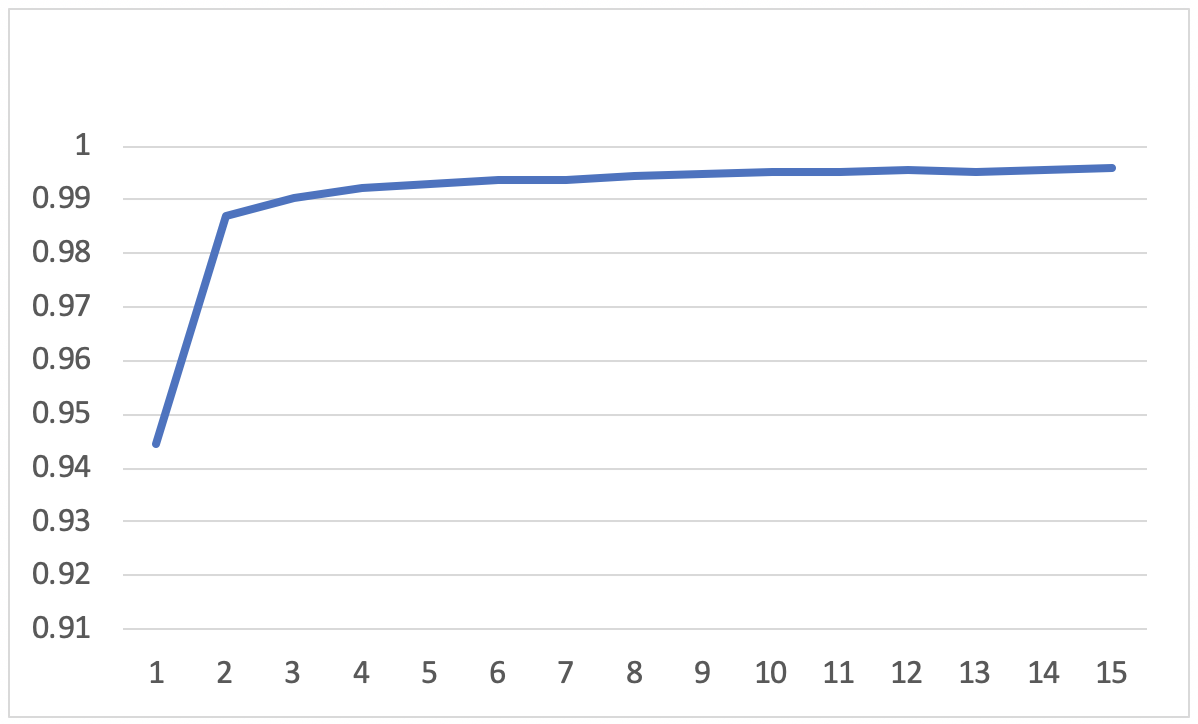
\includegraphics[width=7cm]{figures/cnn/training/accuracy.png}
		\caption{صحت شبکه دسته‌بند}
		\label{fig:cnn_training_acc}
	\end{figure}
	\columnbreak
	\begin{figure}[H]
		\centering
		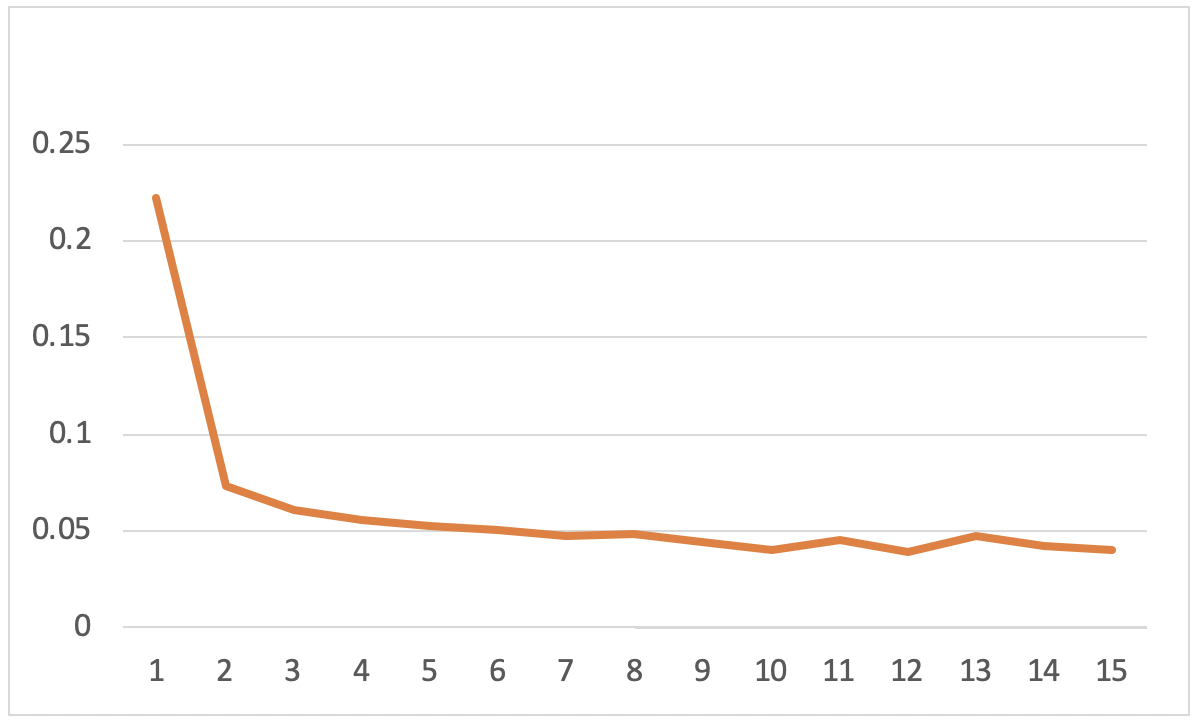
\includegraphics[width=7cm]{figures/cnn/training/loss.png}
		\caption {هزینه‌ی شبکه دسته‌بند}
		\label{fig:cnn_training_loss}
	\end{figure}
\end{multicols}

\noindent در جدول \ref{tab:cnn_evaluation} نتایج ارزیابی دسته‌بند شبکه عصبی پیچشی را مشاهده می‌کنید. از آنجا که روش تعبیه‌سازی استفاده شده در این دسته‌بند یعنی روش \lr{word2vec}، یکی از روش‌های تعبیه‌سازی مورد استفاده در دسته‌بند ماشین بردار پشتبیان نیز می‌باشد، برای مقایسه، نتایج آزمایش مربوط به این روش تعبیه‌سازی در دسته‌بند ماشین بردار پشتبیان که در جدول \ref{tab:svm_evaluation} بیان شدند در جدول \ref{tab:cnn_evaluation} نیز آورده شده‌اند.
با مقایسه‌ی نتایج این دو دسته‌بند مشخص می‌شود که در اکثر آزمایش‌ها و روش‌ها شبکه عصبی پیچشی عملکرد نسبتاً بهتری را داشته است.
\begin{table}[h]
	\centering
	\def\arraystretch{0.85}
	\setlength{\tabcolsep}{9pt}
	\begin{tabular}{|c|c|>{\setlatin}c|>{\setlatin}c|>{\setlatin}c|>{\setlatin}c|}
		\hline
		\rowcolor{headerColor}
		& & & دقت & فراخوانی & 
		\\
		\rowcolor{headerColor}
		\multirow{-2}{*}{روش آزمایش}&\multirow{-2}{*}{نوع دسته‌بند}&\multirow{-2}{*}{~صحت~}&(میانگین ماکرو)&(میانگین ماکرو)&\multirow{-2}{*}{امتیاز $F_{1}$}
		\\ \hline
	
		&\lr{CNN}&\begin{tabular}{@{}c@{}c@{}}‌~\\99.72\\~\end{tabular}&99.55&99.49&99.52
		\\
		\multirow{-4}{*}{۵تایی}
		&\lr{SVM}&\begin{tabular}{@{}c@{}c@{}}‌~\\99.63\\~\end{tabular}&99.35&99.31&99.33
		\\ \hline
		
		&\lr{CNN}&\begin{tabular}{@{}c@{}c@{}}‌~\\99.66\\~\end{tabular}&99.44&99.37&99.40
		\\
		\multirow{-4}{*}{مجموعه داده}
		&\lr{SVM}&\begin{tabular}{@{}c@{}c@{}}‌~\\99.46\\~\end{tabular}&99.16&98.89&99.02
		\\ \hline
		
		&\lr{CNN}&\begin{tabular}{@{}c@{}c@{}}‌~\\98.24\\~\end{tabular}&96.49&96.63&96.56
		\\
		\multirow{-4}{*}{\begin{tabular}{@{}c@{}}مجموعه داده\\الگو متمایز\end{tabular}}
		&\lr{SVM}&\begin{tabular}{@{}c@{}c@{}}‌~\\98.57\\~\end{tabular}&97.54&97.19&97.36
		\\ \hline
		
		&\lr{CNN}&\begin{tabular}{@{}c@{}c@{}}‌~\\99.60\\~\end{tabular}&99.49&99.32&99.40
		\\
		\multirow{-4}{*}{\begin{tabular}{@{}c@{}}مجموعه داده\\یک‌جهته\end{tabular}}
		&\lr{SVM}&\begin{tabular}{@{}c@{}c@{}}‌~\\98.95\\~\end{tabular}&98.37&98.10&98.23
		\\ \hline
		
		&\lr{CNN}&\begin{tabular}{@{}c@{}c@{}}‌~\\96.65\\~\end{tabular}&93.69&93.20&93.45
		\\ 
		\multirow{-4}{*}{\begin{tabular}{@{}c@{}c@{}}مجموعه داده\\یک‌جهته\\الگو متمایز\end{tabular}}
		&\lr{SVM}&\begin{tabular}{@{}c@{}c@{}}‌~\\95.96\\~\end{tabular}&92.67&92.86&92.76
		\\ \hline
	\end{tabular}	
	\caption[ارزیابی دسته‌بندها در روش تعبیه‌سازی \lr{word2vec}]{ارزیابی دسته‌بند شبکه عصبی پیچشی و ماشین بردار پشتیبان که از روش تعبیه‌سازی \lr{word2vec} استفاده کرده‌اند. این دو دسته‌بند به اختصار و به ترتیب با نام‌های \lr{CNN} و \lr{SVM} در جدول بیان شده‌اند.}
	\label{tab:cnn_evaluation}
\end{table}	
\\
نمونه‌هایی از داده‌های مشکل دار دسته‌بند شبکه عصبی پیچشی استخراج شده‌اند که در جدول \ref{tab:cnn_troubled_samples} قرار دارند. مشکل نمونه‌ی دوم و آخر مشابه بودن کلمات مربوط به هر دو رابطه است. اما مشکل نمونه‌های اول، سوم و چهارم در این است که کلمات "اولیاء"، "بازیگرانش" و "مساحتش" در جملات آموزش حضور نداشته‌اند. این مشکل با انجام که پیش‌پردازش و ریشه‌یابی کلمات تا حدود قابل توجهی قابل حل می‌باشد. در این صورت به عنوان مثال کلمه‌ی "بازیگرانش" با کلمه‌ی "بازیگر" جایگزین می‌شود که در کلمات آموزش حضور داشته است.
\begin{table}[h]
	\centering
	\def\arraystretch{1.7}
	\begin{tabularx}{\linewidth}{|L|c|c|}
		\hline
		\rowcolor{headerColor}
		\multicolumn{1}{|c|}{پرسش}&رابطه‌ی هدف&رابطه‌ی تشخیص داده شده
		\\ \hline
		\small{اولیاء یاپ کوهن را نام ببرید}&آثار یک شخص&فرزندان یک شخص
		\\ \hline
		\small{نفوس خون کاین چند نفر است}&جمعیت&جمعیت یک کشور
		\\ \hline
		\small{سریال تلویزیونی معالجه با شوک (فیلم ۱۹۷۳) بازیگرانش کدامند}& بازیگران یک سریال تلویزیونی&کارگردان یک سریال تلویزیونی
		\\ \hline
		\small{گمینا تژچیل مساحتش چقدر است}&مساحت یک کشور&درامد
		\\ \hline
		\small{چه کسی سریال تلویزیونی دکتر اورلوف افتضاح را کارگردانی می کند}&کارگردان یک سریال تلویزیونی&کارگردان یک فیلم
		\\ \hline
	\end{tabularx}	
	\caption{نمونه‌های مشکل‌دار دسته‌بند شبکه عصبی پیچشی}
	\label{tab:cnn_troubled_samples}
\end{table}
\\
هرچند هدف دسته‌بند رابطه در این سیستم تشخیص یک رابطه بوده و تک کلاسه می‌باشد و بدین صورت آموزش دیده‌ است اما از دسته‌بند ماشین بردار پشتیبان می‌توان انتظار تشخیص دو یا چند رابطه‌ی مرتبط را داشت. به عنوان نمونه این دسته‌بند برای پرسش "زبان و پایتخت کشور ایران چیست" رابطه‌ی "پایتخت یک کشور" را با احتمال ۶۴\lr{\%} و رابطه‌ی "زبان رسمی یک کشور" را با احتمال ۳۱\lr{\%} تشخیص می‌دهد. در صورتی که دسته‌بند شبکه عصبی پیچشی برای همین پرسش رابطه‌ی "پایتخت یک کشور" را با احتمال ۹۹\lr{\%} تشخیص داده و برای بقیه‌ی روابط احتمال بسیار کمی تولید می‌کند. با جا به جا کردن کلمات همین پرسش و تغییر آن به جمله‌ی "پایتخت و زبان کشور ایران چیست" مشاهده می‌شود که نتیجه‌ی دسته‌بند شبکه عصبی پیچشی تغییر کرده و این بار رابطه‌ی "زبان رسمی یک کشور" را با احتمال ۱۰۰\lr{\%} تشخیص می‌دهد. دلیل این عملکرد پیچیده‌تر بودن این شبکه نسبت به دسته‌بند ماشین بردار پشتیبان و آموزش آن برای هدف تک کلاسه می‌باشد.
\subsection{ارزیابی کتابخانه‌ی تشخیص‌دهنده موجودیت‌های نام‌دار}
یکی از روش‌های گفته شده برای استخراج موجودیت‌های جملات در این سیستم استفاده از کتابخانه‌ی پیاده شده در آزمایشگاه پردازش زبان‌های طبیعی امیرکبیر می‌باشد. ارزیابی این قسمت در دو سطح توکن\footnote{\lr{Token Level}} و عبارت\footnote{\lr{Phrase Level}} انجام شده است. در سطح توکن، برچسب\footnote{\lr{Tag}}‌های پیش‌بینی شده توسط مدل با برچسب‌های صحیح آن به طور مستقل برای هر کلمه مقایسه می‌شود. این برچسب‌ها می‌توانند نشان‌دهنده‌ی موجودیت بودن یا نبودن آن کلمه باشند. اما در سطح عبارت در صورتی پاسخ مدل به عنوان پاسخ درست برداشت می‌شود که برچسب‌ تمامی کلمات آن جمله مطابق با برچسب‌های صحیح باشد. در سطح عبارت روش دومی نیز برای ارزیابی پیاده شده که در آن اگر تعداد برچسب‌های تولیدی توسط کتابخانه کمتر از تعداد برچسب‌های مورد انتظار باشد، تعدادی برچسب '\lr{o}' (که نماینده‌ی موجودیت نبودن است) به انتهای برچسب‌ها اضافه می‌شود و سپس برچسب‌های دو عبارت مقایسه می‌شوند. دلیل این روش بر این اساس است که تشخیص ندادن برچسب برای یک کلمه و یا تشخیص موجودیت نبودن برای آن کلمه در عمل برای سیستم تفاوتی ندارد. نتایج این آزمایش را در جداول \ref{tab:ner_evaluation_tag_lvl} و \ref{tab:ner_evaluation_phrase_lvl} مشاهده می‌نمایید. برای این آزمایش از مجموعه داده‌ی الگو متمایز که در بخش پیشین معرفی شد استفاده شده است.
\begin{table}[h]
	\centering
	\def\arraystretch{1.3}
	\setlength{\tabcolsep}{12pt}
	\begin{tabular}{|>{\setlatin}C{1.5cm}|>{\setlatin}C{1.5cm}|>{\setlatin}C{1.5cm}|>{\setlatin}C{1.5cm}|}
		\hline
		\rowcolor{headerColor}
		صحت&دقت&فراخوانی&امتیاز $F_{1}$
		\\ \hline
		95.13&100&80.72&89.33
		\\ \hline
	\end{tabular}	
\caption{ارزیابی کتابخانه‌ی تشخیص‌دهنده موجودیت‌های نام‌دار در سطح توکن}
\label{tab:ner_evaluation_tag_lvl}
\end{table}

\begin{table}[h]
	\centering
	\def\arraystretch{1.3}
	\setlength{\tabcolsep}{12pt}
	\begin{tabular}{|c|>{\setlatin}C{1.5cm}|}
		\hline
		\rowcolor{headerColor}
		ورودی&صحت
		\\ \hline
		برچسب تولید شده&67.30
		\\ \hline
		برچسب تکمیل شده&79.42
		\\ \hline
	\end{tabular}	
	\caption{ارزیابی کتابخانه‌ی تشخیص‌دهنده موجودیت‌های نام‌دار در سطح عبارت}
	\label{tab:ner_evaluation_phrase_lvl}
\end{table}

نمونه‌هایی از داد‌ه‌هایی که این کتابخانه در تشخیص برچسب‌های آنان مشکل داشته را در جدول \ref{tab:ner_troubled_samples} مشاهده می‌کنید. برچسب '\lr{o}' نماینده‌ی موجودیت نبودن و برچسب '\lr{i}' نماینده‌ی موجودیت بودن است. یکی از ایرادات این کتابخانه که در موارد زیادی منجر به اشتباه شده، تشخیص اشتباه کلمات پایانی سوالات مانند "می‌باشد"، "است"، "چه کسی" و "چیست" به عنوان موجودیت است.

\begin{table}[h]
	\centering
	\def\arraystretch{1.5}
	%\setlength{\tabcolsep}{12pt}
	\begin{tabularx}{\linewidth}{|L|C{3cm}|C{3cm}|}
		\hline
		\rowcolor{headerColor}
		\multicolumn{1}{|c|}{پرسش}
		&برچسب هدف&برچسب تشخیص داده شده
		\\ \hline
		چه آثاری مربوط به شخص جاد اپتاو می باشند&\lr{oooooiioo}&\lr{ooooooooo}
		\\ \hline
		انتشار چه کتابی توسط نشر اکتیویژن انجام گرفته است&\lr{oooooiooo}&\lr{oooooiiii}
		\\ \hline
		والدین جفری (1952-2014) را نام ببرید&\lr{oiiooo}&\lr{iiiooo}
		\\ \hline
		ملیت شخص سالی فیلیپس چه نام دارد&\lr{ooiiooo}&\lr{oooiooo}
		\\ \hline
		ریاست اداره شهرداری سن-فردیناند، کبک در حال حاضر از ان چه شخصی است&\lr{oooiioooooooo}&\lr{oooiiooooooii}
		\\ \hline
		سازنده آهنگ فیلم تروریسم (فیلم ۱۹۹۷) چه کسی است&\lr{oooiiiooo}&\lr{oooiiiiii}
		\\ \hline
		پلاک خودروهای شهر داننبرگ (الب) چند است&\lr{oooiioo}&\lr{oooiioi}
		\\ \hline
		آثار حسین مسرور چه نام دارند&\lr{oiiooo}&\lr{oioooo}
		\\ \hline
		\setlatin{457.36} رنمینبی میلیارد رنمینبی تومان میزان متوسط درآمد سالیانه کدام شرکت است&\lr{iiiioooooooo}&\lr{iiiiiiiiiiii}
		\\ \hline
		مولفی که حکایت‌نامه (لطائف المتون) را نگارش کرده است کیست&\lr{ooiiiooooo}&\lr{ooiiiiiiii}
		\\ \hline
		نام نگارنده ای که اثر تاریخ حقوق ایران را نگارش کرده است چیست&\lr{oooooiiiooooo}&\lr{oooooiiiooooi}
		\\ \hline
	\end{tabularx}	
	\caption[نمونه‌های مشکل‌دار کتابخانه‌ی تشخیص‌دهنده موجودیت‌های نام‌دار]{نمونه‌های مشکل‌دار کتابخانه‌ی تشخیص‌دهنده موجودیت‌های نام‌دار (ستون‌های دوم و سوم چپ به راست می‌باشند)}
	\label{tab:ner_troubled_samples}
\end{table}

\subsection{ارزیابی یکپارچه‌ی سیستم}
برای ارزیابی یکپارچه‌ی سیستم ۱۰\lr{\%} از مجموعه داده‌ی اصلی (حدود ۶۵۰۰ داده) تحت عنوان مجموعه‌ی آزمایش جدا شده و بوسیله‌ی آنها ارزیابی انجام می‌شود. در این ارزیابی اولین رابطه‌ی تشخیص داده شده توسط دسته‌بند و اولین موجودیت تشخیص داده شده در جمله استفاده شده و کوئری به پایگاه دانش ارسال می‌گردد. در صورتی آن داده‌ی آزمون موفقیت‌آمیز تلقی می‌شود که موجودیت پاسخ هدف در مجموعه موجودیت‌های دریافت شده از پایگاه دانش باشد. از آنجا که دسته‌بندها جداگانه آزمایش شده‌اند،‌ در این ارزیابی دسته‌بندهای مورد استفاده روی کلیه‌ی داده‌ها آموزش دیده‌اند تا بهترین عملکرد خود را داشته باشند. برای تشخیص موجودیت‌ها نیز از هر دو روش توضیح داده شده در بخش تشخیص موجودیت‌ها در فصل چهارم استفاده شده است.
در جدول \ref{tab:end2end_evaluation} نتایج این ارزیابی را که طی دو آزمایش با دسته‌بندهای مختلف انجام شده‌اند مشاهده می‌نمایید.

\begin{table}[h]
	\centering
	\def\arraystretch{1.5}
	\setlength{\tabcolsep}{12pt}
	\begin{tabular}{|c|>{\setlatin}C{1.5cm}|}
		\hline
		\rowcolor{headerColor}
		نوع دسته‌بند&صحت
		\\ \hline
		ماشین بردار پشتیبان & \multirow{2}{*}{28.47}
		\\
		(\lr{word2vec} وزن‌دار) &
		\\ \hline
		\multirow{2}{*}{شبکه عصبی پیچشی}&\multirow{2}{*}{29.07}
		\\
		&
		\\ \hline
	\end{tabular}	
	\caption{ارزیابی یکپارچه‌ی سیستم}
	\label{tab:end2end_evaluation}
\end{table}
با بررسی نتایج این آزمایش مشخص می‌شود که در حدود ۲۳.۸۰\lr{\%} موارد دسته‌بند رابطه و کتابخانه‌ی تشخیص‌دهنده موجودیت‌های نام‌دار عملکرد صحیحی داشته‌اند. بنابراین در حدود ۵۰.۵۱\lr{\%} موارد با آنکه رابطه و برچسب‌های تشخیص داده شده صحیح بوده‌اند اما در نهایت پاسخ صحیح دریافت نشده است که نشان می‌دهد عمده‌ی مشکل در عملکرد پایگاه دانش فارس‌بیس می‌باشد. ناموفق بودن این ‌موارد در علل زیر خلاصه می‌شوند:
\begin{itemize}
	\item
	 برخی از موجودیت‌ها دارای کلمات مشابه با موجودیت‌های دیگری هستند. در برخی از این موارد پایگاه دانش گره‌ی نادرستی از پایگاه را به کلمه‌ی مورد نظر نگاشت می‌کند. مانند:
		\begin{itemize} 
			\item قندهار پایتخت کدام کشور است
				\begin{itemize} 
					\small
					\item گره صحیح: 
					\href{http://fkg.iust.ac.ir/resource/\%D9\%82\%D9\%86\%D8\%AF\%D9\%87\%D8\%A7\%D8\%B1}
{قندهار}
					\item گره نگاشت شده:
					\href{http://fkg.iust.ac.ir/resource/\%D9\%82\%D9\%86\%D8\%AF\%D9\%87\%D8\%A7\%D8\%B1\_\%28\%D9\%85\%D9\%84\%DA\%A9\%D8\%A7\%D9\%86\%29}
					{قندهار\lr{\_}$)$ملکان$($}
			\end{itemize}
			\item نام بازیگران سریال تلویزیونی دایره راز ذکر کنید
				\begin{itemize} 
					\small
					\item گره صحیح: 
					\href{http://fkg.iust.ac.ir/resource/\%D8\%AF\%D8\%A7\%DB\%8C\%D8\%B1\%D9\%87\_\%D8\%B1\%D8\%A7\%D8\%B2}
					{دایره\lr{\_}راز}
					
					\item گره نگاشت شده:
					دو گره‌ی
					\href{http://fkg.iust.ac.ir/resource/\%D8\%AF\%D8\%A7\%DB\%8C\%D8\%B1\%D9\%87}
					{دایره}
					و
					\href{http://fkg.iust.ac.ir/resource/\%D8\%B1\%D8\%A7\%D8\%B2\_\%28\%D8\%B7\%D8\%A7\%DB\%8C\%D9\%81\%D9\%87\%29}
					{راز\lr{\_}$)$طایفه$($}
				به ترتیب به کلمات مرتبط نگاشت شده‌اند.
				\end{itemize}
		\end{itemize}
		\item
در برخی موارد با آنکه موجودیت مورد پرسش در پایگاه وجود دارد اما هیچ گره‌ای به آن نگاشت نمی‌شود. مانند:
		\begin{itemize} 
			\item مقدار پول کسب شده از فروش فیلم رسوایی ۲
			\begin{itemize} 
				\small
				\item گره صحیح: 
				\href{http://fkg.iust.ac.ir/resource/\%D8\%B1\%D8\%B3\%D9\%88\%D8\%A7\%DB\%8C\%DB\%8C\_\%DB\%B2}
				{رسوایی\lr{\_}۲}
			\end{itemize}
			\item اسم فیلمی که \lr{Souheil Ben-Barka} کارگردانش است
			\begin{itemize} 
				\small
				\item گره صحیح: 
				\href{http://fkg.iust.ac.ir/resource/Souheil_Ben-Barka}
				{\lr{Souheil\_Ben-Barka}}
			\end{itemize}
		\end{itemize}
	\item این پایگاه دانش ویژگی‌هایی که به صورت یک عدد (مانند موجودیت‌های مرتبط با سوالات درآمد، مساحت و جمعیت) یا یک آدرس اینترنتی هستند را به صورت یک گره نگه‌داری نمی‌کند و در تشخیص چنین موجودیت‌هایی ناتوان است. مانند:
		\begin{itemize} 
			\item مقدار ۴۰.۷۰ مربوط به مساحت کدام کشور است
			\item سایت \lr{www.kreis-reutlingen.de} متعلق به چه ارگانی است
		\end{itemize}
\end{itemize}
با ارزیابی این نمونه‌های مشکل‌دار مشخص می‌شود که در حدود ۹۲\lr{\%} نمونه‌ها هیچ گره‌ای نگاشت نمی‌شود که مربوط به علل دوم و سوم است و فقط در ۸\lr{\%} موارد نگاشت اشتباه انجام گرفته که مربوط به علت اول در علل ذکر شده می‌باشد.

\subsection{ارزیابی مدل دنباله به دنباله}
در فصل دوم با نوعی شبکه‌ی عصبی به نام شبکه‌ی عصبی دنباله به دنباله آشنا شدیم. در آزمایشگاه پردازش زبان طبیعی امیرکبیر سیستم پرسش و پاسخ دیگری وابسته به پایگاه دانش فارس‌بیس توسعه یافته است که از شبکه عصبی دنباله به دنباله به صورت یکپارچه استفاده می‌کند. ورودی این شبکه یک پرسش و خروجی آن کوئری مرتبط با آن پرسش است که با ارسال آن کوئری به پایگاه دانش فارس‌بیس موجودیت پاسخ مرتبط دریافت می‌گردد \cite{persian_seq2seq}.
در ادامه به ارزیابی مدل دنباله به دنباله و مقایسه‌ی آن با سیستم فعلی موجود در این پروژه می‌پردازیم. در تمامی ارزیابی‌های صورت‌گرفته روی این مدل از مجموعه داده‌ی الگو متمایز که در قسمت ارزیابی دسته‌بندهای رابطه معرفی شد استفاده شده است.
\\
در اولین ارزیابی به بررسی رابطه‌ی شناخته شده توسط این مدل می‌پردازیم. به این منظور کوئری تولید شده توسط این مدل دریافت و شناسه‌ی رابطه از کوئری استخراج شده و با رابطه‌ی هدف مقایسه می‌شود. ‌این ارزیابی صحت ۵۸.۸۳\lr{\%} را نتیجه می‌دهد که همانطور که در جدول \ref{tab:seq2seq_rel_evaluation} مشاهده می‌نمایید دسته‌بندهای استفاده شده در این پروژه عملکرد بهتری را در تشخیص رابطه نشان داده‌اند. در این جدول بهترین نتایج دو دسته‌بند در آزمایش با مجموعه داده‌ی الگو متمایز آورده شده‌اند.
\begin{table}[h]
	\centering
	\def\arraystretch{1.5}
	\setlength{\tabcolsep}{12pt}
	\begin{tabular}{|c|>{\setlatin}C{1.5cm}|}
		\hline
		\rowcolor{headerColor}
		مدل&صحت
		\\ \hline
		دسته‌بند ماشین بردار پشتیبان &98.76
		\\ \hline
		دسته‌بند شبکه عصبی پیچشی&98.24
		\\ \hline
		مدل دنباله به دنباله&83.58
		\\ \hline
	\end{tabular}	
	\caption{مقایسه‌ی مدل دنباله به دنباله و دسته‌بندهای سیستم در تشخیص رابطه}
	\label{tab:seq2seq_rel_evaluation}
\end{table}
\\در ارزیابی دیگر، این مدل به صورت سرتاسری مورد آزمایش قرار می‌گیرد. در این ارزیابی کوئری تولید شده توسط مدل به پایگاه دانش ارسال می‌شود و پاسخ‌های دریافتی با پاسخ هدف مقایسه می‌شوند. از آنجا که کوئری‌های تولید شده توسط مدل دنباله به دنباله نتیجه‌ی ضعیفی را به دنبال داشتند، در چند مرحله مورد بهبود قرار گرفته و دوباره ارزیابی شدند. نقص عمده‌ی این مدل در تشخیص اشتباه شناسه‌ی موجودیت موجود در پرسش می‌باشد که از آنجا که این مدل برای تولید کوئری ارتباطی با پایگاه دانش برقرار نمی‌کند قابل انتظار است. مراحل بهبود این مدل به شرح زیر است:
\begin{itemize}
	\item \textbf{تشخیص موجودیت پرسش:}
ممکن است در کوئری تولید شده شناسه‌ی موجودیت مورد پرسش در پایگاه دانش فارس‌بیس به اشتباه تشخیص داده شده باشد. برای بهبود می‌توان از روش‌های یادشده در این پروژه برای یافتن موجودیت موجود پرسش استفاده کرد و شناسه‌ی آن موجودیت را بوسیله‌ی رابط برنامه‌نویسی کاربردی فارس‌بیس استخراج و در کوئری جایگزین نمود.
	\item \textbf{استفاده از شناسه‌ی موجودیت اصلی:}
	این مرحله جایگزین مرحله‌ی قبل می‌باشد. در این مرحله با استفاده از مجموعه داده‌ها شناسه‌ی موجودیت مورد پرسش مستقیماً استفاده شده و در کوئری قرار داده می‌شود. در صورت استفاده از این مرحله دیگر برای تشخیص شناسه‌ی موجودیت نیاز به رابط برنامه‌نویسی کاربردی فارس‌بیس نمی‌باشد. همانطور که مشخص است، این مرحله در سیستم عملی قابل استفاده نیست و صرفا برای ارزیابی کوئری تولیدی استفاده شده است.
	\item \textbf{بررسی کوئری وارون:} ممکن است شناسه‌ی رابطه و موجودیت پرسش صحیح باشند اما جهت کوئری نادرست باشد. در این مرحله در صورت ناموفق بودن کوئری، جهت کوئری وارون شده و دوباره ارسال و بررسی می‌شود. این مرحله در ادامه‌ی هر دو مرحله‌ی قبلی استفاده می‌شود. 
\end{itemize}
نتایج این ارزیابی را در جدول \ref{tab:seq2seq_evaluation} مشاهده می‌کنید. همانطور که از نتایج مشخص است در بهترین حالت قابل استفاده در سیستم عملی و با استفاده از روش‌های تشخیص موجودیت این پروژه صحت ۹۱.۲۷\lr{\%} بدست می‌آید که نتیجه‌ای مشابه با سیستم پیاده شده در این پروژه دارد. توجه شود که مرحله‌ی استفاده از شناسه‌ی موجودیت اصلی در سیستم عملی قابل استفاده نمی‌باشد. علت اصلی صحت پایین پاسخ‌ها حتی در صورت استفاده از شناسه‌ی موجودیت اصلی، تعداد زیاد نمونه‌هایی می‌باشد که موجودیت حاضر در سوالشان از نوع عدد یا آدرس اینترنتی بوده و به ازای آنها هیچ گره‌ای در پایگاه دانش وجود ندارد. به همین سبب تولید کوئری برای چنین سوالاتی مقدور نمی‌باشد. این نمونه‌ها علت اصلی صحت پایین در ارزیابی یکپارچه‌ی سیستم نیز بوده‌اند که در بخش قبل به طور مفصل شرح داده شدند.
\begin{table}[t]
	\centering
	\def\arraystretch{1.5}
	\setlength{\tabcolsep}{12pt}
	\begin{tabular}{|c|>{\setlatin}C{1.5cm}|}
		\hline
		\rowcolor{headerColor}
		مرحله&صحت
		\\ \hline
		کوئری اصلی&1.33
		\\ \hline
		تشخیص موجودیت پرسش&25.78
		\\ \hline
		تشخیص موجودیت پرسش + بررسی کوئری وارون&27.91
		\\ \hline
		استفاده از شناسه‌ی موجودیت اصلی&38.17
		\\ \hline
		استفاده از شناسه‌ی موجودیت اصلی+ بررسی کوئری وارون&40.67
		\\ \hline
	\end{tabular}	
	\caption{ارزیابی مدل دنباله به دنباله}
	\label{tab:seq2seq_evaluation}
\end{table}
